\documentclass{scalatekids-article}
\usepackage[italian]{babel}
\begin{document}
\lfoot{Specifica Tecnica 1.0.0}
\newgeometry{top=3.5cm}
\begin{titlepage}
  \begin{center}
    \begin{center}
      
\includegraphics[width=10cm]{sklogo.png}
    \end{center}
    \vspace{1cm}
    \begin{Huge}
      \begin{center}
        \textbf{Specifica Tecnica}
      \end{center}
    \end{Huge}
    \vspace{11pt}
    \bgroup
    \def\arraystretch{1.3}
    \begin{tabular}{r|l}
      \multicolumn{2}{c}{\textbf{Informazioni sul documento}} \\
      \hline
      \setbox0=\hbox{0.0.1\unskip}\ifdim\wd0=0pt
      \\
      \else
      \textbf{Versione} & 1.0.0\\
      \fi
      \textbf{Redazione} & \multiLineCell[t]{}\\
      \textbf{Verifica} & \multiLineCell[t]{}\\
      \textbf{Approvazione} & \multiLineCell[t]{}\\
      \textbf{Uso} & Esterno\\
      \textbf{Lista di Distribuzione} & \multiLineCell[t]{ScalateKids\\Prof. Tullio Vardanega\\Prof. Riccardo Cardin}\\
    \end{tabular}
    \egroup
    \vspace{22pt}
  \end{center}
\end{titlepage}
\restoregeometry
\clearpage
\pagenumbering{Roman}
\setcounter{page}{1}
\begin{flushleft}
  \vspace{0cm}
  {\large\bfseries Diario delle modifiche \par}
\end{flushleft}
\vspace{0cm}
\begin{center}
  \begin{tabular}{| l | l | l | l | p{5cm} |}
    \hline
    Versione & Autore & Ruolo & Data & Descrizione \\
    \hline
    0.4.0 & Michael Munaro & Verificatore & 2016-03-25 & Verifica sezione 5\\
    \hline
    0.3.1 & Giacomo Vanin & Progettista & 2016-03-24 & Stesura sezione 5\\
    \hline
    0.3.0 & Alberto De Agostini & Verificatore & 2016-03-22 & Verifica sezioni da 4.6 a 4.13\\
    \hline
    0.2.2 & Marco Boseggia & Progettista & 2016-03-22 & Stesura sezioni 4.10 4.11 4.12 4.13\\
    \hline
    0.2.1 & Marco Boseggia & Progettista & 2016-03-21 & Stesura sezioni 4.6 4.7 4.8 4.9\\
    \hline
    0.2.0 & Michael Munaro & Verificatore & 2016-03-21 & Verifica sottosezioni 3.1 3.2 4.1 4.2 4.3 4.4 4.5\\
    \hline
    0.1.2 & Andrea Giacomo Baldan & Progettista & 2016-03-17 & Stesura sottosezioni 4.1 4.2 4.3 4.4 4.5\\
    \hline
    0.1.1 & Andrea Giacomo Baldan & Progettista & 2016-03-17 & Stesura sottosezioni 3.1 3.2\\
    \hline
    0.1.0 & Michael Munaro & Verificatore & 2016-03-16 & Verifica sezioni 1 e 2\\
    \hline
    0.0.2 & Marco Boseggia & Progettista & 2016-02-26 & Stesura sezioni 1 e 2\\
    \hline
    0.0.1 & Andrea Giacomo Baldan & Amministratore & 2016-02-26 & Creazione scheletro del documento\\
    \hline
  \end{tabular}
\end{center}
\tableofcontents
\newpage
\pagenumbering{arabic}

\section{Sommario}

\subsection{Scopo del documento}

Il seguente documento ha lo scopo di descrivere la progettazione ad alto livello
che il gruppo \textit{ScalateKids} ha scelto per il
progetto\textbf{ActorBase}.\\  Sarà descritta l'\gloss{architettura} generale
del progetto, in particolare  la scelta dei \gloss{design pattern} e delle
componentiche andranno a comporre il software.

\prodPurpose

\glossExpl

\subsection{Riferimenti}

\subsubsection{Normativi}

\begin{itemize}

\item\textbf{Capitolato d'appalto C1:} \textit{Actorbase: a
NoSQL DB based on the Actor model;}\\
\url{http://www.math.unipd.it/~tullio/IS-1/2015/Progetto/C1.pdf}
\item\textbf{Norme di Progetto:}
\href{run:../Interni/NormeDiProgetto\_v2.0.0.pdf}{Norme di Progetto v2.0.0.}
\end{itemize}

\subsubsection{Informativi}

\begin{itemize}
\item\textbf{Piano di Progetto:}
\href{run:./PianoDiProgetto\_v2.0.0.pdf}{Piano di Progetto v2.0.0}
\item\textbf{Dispense fornite dall'insegnamento Ingegneria del Software mod.
A:}\\   \url{http://www.math.unipd.it/~tullio/IS-1/2015/}
\item\textbf{Documentazione di \gloss{Akka} su \gloss{Scala}:}
\url{http://doc.akka.io/docs/akka/2.4.2/scala.html}
\end{itemize}

\newpage

\section{Tecnologie utilizzate}

In questa sezione saranno descritte le tecnologie scelte per lo sviluppo del
progetto \textbf{ActorBase} e le motivazioni che ci hanno spinto a sceglierle.

\subsection{Akka}

La scelta della libreria \gloss{Akka} è stata dettata dal capitolato. Tuttavia
l'avremmo scelta comunque per i seguenti motivi:
\begin{itemize}
\item\textbf{Implementazione del \gloss{modello ad attori}:} \gloss{Akka}
rende semplice la creazione e l'utilizzo degli \gloss{attori}. Grazie a ciò
viene naturale la distribuibilità del progetto e l'asincronia tra i processi;
\item\textbf{Tolleranza agli errori:} \gloss{Akka} implementa un sistema di
gerarchia di supervisori. Questa gerarchia consente ai supervisori di un
\gloss{attore}, nel caso in cui quest'ultimo lanci un'eccezione, di mandarlo
in \gloss{crash} e farlo poi ripartire. In questo modo il sistema è resiliente
agli errori;
\item\textbf{Persistenza:} Ogni messaggio ricevuto da ciascun \gloss{attore}
può essere salvato in maniera tale che al riavvio esso possa riprendere da
dov'era prima del suo spegnimento.
\end{itemize}

\subsection{Scala}

Il capitolato richiede l'utilizzo di un linguaggio di programmazione a scelta
tra \gloss{Scala} e \gloss{Java}. Abbiamo scelto \gloss{Scala} per i seguenti
motivi:

\begin{itemize}
\item\textbf{gloss{Programmazione funzionale}:} Questa tecnica di
programmazione evita che ci siano degli effetti collaterali tra funzioni,
rendendole quindi gloss{thread-safe};
\item\textbf{Implementazione di gloss{Akka}:} gloss{Akka} risulta più
facilmente implementabile in gloss{Scala} che in gloss{Java}. Questo perchè
la \gloss{programmazione funzionale} con i suoi paradigmi si integra meglio
con il gloss{modello ad attori};%%TODO completare lista
\end{itemize}

\section{Descrizione architettura}

\subsection{Metodo e formalismo di specifica}

L'approccio alla progettazione è stato meet-in-the-middle, la prima
suddivisione ad alto livello è stata tra sistema come struttura ad attori e
componenti esterne per utilizzare la base di dati (operazioni CRUD).

\subsection{Architettura generale}

Macroscopicamente il sistema si suddivide in due componenti principali,
assimilabili ad un paradigma Client-Server, il sistema ad attori dove
risiedono la struttura della base di dati ed un server TCP pronto a ricevere
comandi dall'esterno rappresentano la componente server, la Command Line
Interface (CLI) rappresenta la componente client mediante la quale è possibile
inviare comandi al sistema e ricevere l'output prodotto da essi, essa farà uso
della componente \gloss{driver} per comunicare con il sistema lato server
mediante un protocollo di comunicazione appositamente creato.

\begin{figure}[H]
  \begin{center}
    \includegraphics[width=0.2\textwidth,keepaspectratio]{RP/RP-ClientServer.png}
    \caption{Diagramma architettura generale}
  \end{center}
\end{figure}

% TODO:
% \begin{figure}
%   \centering

%   \caption{Architettura generale - vista package}
%   \label{fig:architetturaGeneralePackage}
% \end{figure}
%TODO: sta roba è da cancellare ve?
L'intero sistema è rappresentabile mediante una variante del design pattern
\gloss{MVC}, le tre componenti principali si prestano naturalmente
all'assegnazione delle tre parti che formano il design pattern, con la
differenza rispetto ad un approccio più classico, che l'aggiornamento della
parte \gloss{view} avviene sempre e comunque passando per la parte controller,
ciò è dovuto alla natura client-server del prodotto, che richiede un protocollo
di comunicazione ben preciso tra le due parti. Il sistema formato dai package
dedicati agli attori \gloss{akka} e dal server \gloss{TCP} per la comunicazione
con l'esterno sono assimilabili alla parte \gloss{model}, rappresenta la
\gloss{business logic} di \textbf{Actorbase}. La \gloss{CLI} è assimilabile alla
parte \gloss{view}, unico punto di interazione con l'utente, si occupa di
processare i comandi in input e restituire l'output opportunamente formattato,
la componente \gloss{driver} fa da ponte di comunicazione tra \gloss{CLI} e
server, occupandosi della ``traduzione'' dei comandi input secondo il protocollo
di comunicazione scelto, rappresenta la parte \gloss{controller}.

\section{Componenti}

\subsection{actorbase}
\label{sec:actorbase}

% TODO:
% \begin{figure}
%   \centering

%   \caption{Componente Actorbase}
%   \label{fig:componenteActorbase}
% \end{figure}

\subsubsection{Descrizione}

La componente principale rappresentata dal package globale \textbf{actorbase}.

\subsubsection{Package contenuti}

\begin{itemize}
\item \hyperref[sec:actorbase::cli]{actorbase::cli};
\item \hyperref[sec:actorbase::driver]{actorbase::driver};
\item \hyperref[sec:actorbase::actorsystem]{actorbase::actorsystem}.
\end{itemize}

Rappresentano le tre macro-componenti del sistema.

\subsection{actorbase::model}
\label{sec:actorbase::model}

\subsubsection{Descrizione}

\gloss{Package} per la componente \gloss{Model} dell'architettura \gloss{MVC},
rappresenta anche la componente system del prodotto.

\subsubsection{Package contenuti}

\begin{itemize}
\item system.
\end{itemize}

\subsection{actorbase::model::system}
\label{sec:actorbase::model::system}

\subsubsection{Descrizione}

\gloss{Package} per la componente system del prodotto.

\subsubsection{Package contenuti}

\begin{itemize}
\item actorbase::model::system::server;
\item actors.
\end{itemize}

\subsection{actorbase::model::system::actors}

\subsubsection{Descrizione}

\gloss{Package} contenente gli \gloss{attori} che agiranno sul \gloss{database}.

\subsubsection{Interazioni con altre componenti}

\begin{itemize}
\item actorbase::model::system::server.
\end{itemize}

\subsubsection{Classi}

\paragraph{actorbase::model::system::actors::Warehouseman}

\subparagraph{Descrizione}

Classe che rappresenta un \gloss{attore} di tipo \gloss{Warehouseman}.

\subparagraph{Utilizzo}

Viene utilizzata per effettuare il salvataggio su filesystem del
\gloss{database}.

\subparagraph{Classi ereditate}

\begin{itemize}
\item actorbase::model::system::actors::Actor.
\end{itemize}

\subparagraph{Interazioni con altre classi}

\begin{itemize}
\item actorbase::model::system::actors::Persistence.
\end{itemize}

\paragraph{actorbase::model::system::actors::Persistence}

\subparagraph{Descrizione}

Interfaccia che consente il salvataggio su filesystem.

\subparagraph{Utilizzo}

Viene utilizzata per offrire un'interfaccia per il salvataggio su filesystem.

\subparagraph{Interazioni con altre classi}

\begin{itemize}
\item actorbase::model::system::actors::Warehouseman.
\end{itemize}

\paragraph{actorbase::model::system::actors::BSONPersistence}

\subparagraph{Descrizione}

Classe che consente di salvare su filesystem in formato \gloss{BSON}.

\subparagraph{Utilizzo}

Viene utilizzata per effettuare il salvataggio su filesystem in formato
\gloss{BSON} del \gloss{database}.

\subparagraph{Classi ereditate}

\begin{itemize}
\item actorbase::model::system::actors::Persistence.
\end{itemize}

\paragraph{actorbase::model::system::actors::Storefinder}

\subparagraph{Descrizione}

Classe che rappresenta un \gloss{attore} di tipo \gloss{Storefinder}.

\subparagraph{Utilizzo}

Viene utilizzata per tenere traccia dei contenuti degli attori di tipo
\gloss{Storekeeper}.

\subparagraph{Classi ereditate}

\begin{itemize}
\item actorbase::model::system::actors::Actor.
\end{itemize}

\paragraph{actorbase::model::system::actors::MainActor}

\subparagraph{Descrizione}

Classe che rappresenta un \gloss{attore} di tipo \gloss{MainActor}.

\subparagraph{Utilizzo}

Viene utilizzata per tenere traccia dei contenuti degli attori di tipo
\gloss{Storefinder}.

\subparagraph{Classi ereditate}

\begin{itemize}
\item actorbase::model::system::actors::Storefinder.
\end{itemize}

\paragraph{actorbase::model::system::actors::Storekeeper}

\subparagraph{Descrizione}

Classe che rappresenta un \gloss{attore} di tipo \gloss{Storekeeper}.

\subparagraph{Utilizzo}

Viene utilizzata per contenere gli elementi all'interno del \gloss{database}.

\subparagraph{Classi ereditate}

\begin{itemize}
\item actorbase::model::system::actors::Actor.
\end{itemize}

\paragraph{actorbase::model::system::actors::Manager}

\subparagraph{Descrizione}

Classe che rappresenta un \gloss{attore} di tipo \gloss{Manager}.

\subparagraph{Utilizzo}

Viene utilizzata per effettuare procedure di \gloss{load balancing}.

\subparagraph{Classi ereditate}

\begin{itemize}
\item actorbase::model::system::actors::Actor.
\end{itemize}

\paragraph{actorbase::model::system::actors::Ninja}

\subparagraph{Descrizione}

Classe che rappresenta un \gloss{attore} di tipo \gloss{Ninja}.

\subparagraph{Utilizzo}

Viene utilizzata per consentire di effettuare un \gloss{backup} dei contenuti
degli attori di tipo \gloss{Storekeeper}.

\subparagraph{Classi ereditate}

\begin{itemize}
\item actorbase::model::system::actors::Actor.
\end{itemize}

\subsection{actorbase::controller}

\subsubsection{Descrizione}

\gloss{Package} per la componente gloss{Controller} dell'architettura
\gloss{MVC}.

\subsubsection{Package contenuti}

\begin{itemize}
\item driver.
\end{itemize}

\subsection{actorbase::controller::driver}

\subsubsection{Descrizione}

\gloss{Package} per la componente \gloss{driver} del prodotto.

\subsubsection{Package contenuti}

\begin{itemize}
\item client;
\item controls;
\item data.
\end{itemize}

\subsection{actorbase::controller::driver::client}

\subsubsection{Descrizione}

\gloss{Package} per la componente client del \gloss{driver} del
\gloss{controller}.

\subsubsection{Interazioni con altre componenti}

\begin{itemize}
\item actorbase::model::system::server;
\item actorbase::view::cli.%TODO giusto?
\end{itemize}

\subsubsection{Classi}

\paragraph{actorbase::controller::driver::client::ActorbaseClient}

\subparagraph{Descrizione}

Classe che rappresenta un'istanza del \gloss{driver}.

\subparagraph{Interazioni con altre classi}

\begin{itemize}
\item actorbase::cli::models::Command;
\item actorbase::controller::driver::client::Connection;
\item actorbase::controller::driver::controls::Control.
\end{itemize}

\paragraph{actorbase::controller::driver::client::Connection}

\subparagraph{Descrizione}

Classe per la connessione tra il \gloss{driver} e il \gloss{server}

\subparagraph{Interazioni con altre classi}
\begin{itemize}
\item actorbase::controller::driver::client::ActorbaseClient;
\item actorbase::model::system::server::TCPServer.
\end{itemize}

\subsection{actorbase::controller::driver::controls}

\subsubsection{Descrizione}

Componente del \gloss{controller} per l'esecuzione del comando e l'interazione
con il \gloss{server}.

\subsubsection{Interazioni con altre componenti}

\begin{itemize}
\item actorbase::model::system::server.
\end{itemize}

\subsubsection{Classi}

\paragraph{actorbase::controller::driver::controls::Control}

\subparagraph{Descrizione}

Interfaccia generica che rappresenta un comando.

\subparagraph{Utilizzo}

Viene utilizzata per offrire un'interfaccia comune a tutti i comandi.

\subparagraph{Interazioni con altre classi}

\begin{itemize}
\item actorbase::controller::driver::client::ActorbaseClient;
\item actorbase::model::system::server::TCPServer.
\end{itemize}

\paragraph{actorbase::controller::driver::controls::FindControl}

\subparagraph{Descrizione}

Classe per il comando di ricerca.

\subparagraph{Utilizzo}

Viene utilizzata per mandare al \gloss{server} il comando di ricerca con i
parametri immessi dall'utente.

\subparagraph{Classi ereditate}

\begin{itemize}
\item actorbase::controller::driver::controls::Control.
\end{itemize}

\paragraph{actorbase::controller::driver::controls::LogoutControl}

\subparagraph{Descrizione}

Classe per il comando di logout.

\subparagraph{Utilizzo}

Viene utilizzata per mandare al \gloss{server} il comando di logout.

\subparagraph{Classi ereditate}

\begin{itemize}
\item actorbase::controller::driver::controls::Control.
\end{itemize}

\paragraph{actorbase::controller::driver::controls::ResetPasswordControl}

\subparagraph{Descrizione}

Classe per il comando di reset della password.

\subparagraph{Utilizzo}

Viene utilizzata per mandare al \gloss{server} il comando di reset della
password dell'utente specificato in input.

\subparagraph{Classi ereditate}

\begin{itemize}
\item actorbase::controller::driver::controls::Control.
\end{itemize}

\paragraph{actorbase::controller::driver::controls::ListControl}

\subparagraph{Descrizione}

Classe per il comando di visualizzazione dell'elenco dei nomi di tutte le
collezioni presenti nel \gloss{database}.

\subparagraph{Utilizzo}

Viene utilizzata per mandare al \gloss{server} il comando di visualizzazione
dell'elenco dei nomi di tutte le collezioni presenti nel \gloss{database}.

\subparagraph{Classi ereditate}

\begin{itemize}
\item actorbase::controller::driver::controls::Control.
\end{itemize}

\paragraph{actorbase::controller::driver::controls::AddContributorControl}

\subparagraph{Descrizione}

Classe per il comando di aggiunta collaboratore a una collezione.

\subparagraph{Utilizzo}

Viene utilizzata per mandare al \gloss{server} il comando di aggiunta di un
collaboratore a una collezione con il nome della \gloss{collezione} e lo
username specificati in input.

\subparagraph{Classi ereditate}

\begin{itemize}
\item actorbase::controller::driver::controls::Control.
\end{itemize}

\paragraph{actorbase::controller::driver::controls::LoginControl}

\subparagraph{Descrizione}

Classe per il comando di login.

\subparagraph{Utilizzo}

Viene utilizzata per mandare al \gloss{server} il comando di login con le
credenziali immesse dall'utente.

\subparagraph{Classi ereditate}

\begin{itemize}
\item actorbase::controller::driver::controls::Control.
\end{itemize}

\paragraph{actorbase::controller::driver::controls::DeleteControl}

\subparagraph{Descrizione}

Classe per il comando di rimozione una \gloss{collezione}.

\subparagraph{Utilizzo}

Viene utilizzata per mandare al \gloss{server} il comando di rimozione di una
collezione con i parametri specificati in input.

\subparagraph{Classi ereditate}

\begin{itemize}
\item actorbase::controller::driver::controls::Control.
\end{itemize}

\paragraph{actorbase::controller::driver::controls::RemoveContributorControl}

\subparagraph{Descrizione}

Classe per il comando di rimozione di un collaboratore da una collezione.

\subparagraph{Utilizzo}

Viene utilizzata per mandare al \gloss{server} il comando di rimozione di un
collaboratore da una collezione con con il nome della \gloss{collezione} e lo
username specificati in input.

\subparagraph{Classi ereditate}

\begin{itemize}
\item actorbase::controller::driver::controls::Control.
\end{itemize}

\paragraph{actorbase::controller::driver::controls::RenameControl}

\subparagraph{Descrizione}

Classe per il comando rinominazione di un item.

\subparagraph{Utilizzo}

Viene utilizzata per mandare al \gloss{server} il comando di rinominazione di
un \gloss{item} con i parametri specificati in input.

\subparagraph{Classi ereditate}

\begin{itemize}
\item actorbase::controller::driver::controls::Control.
\end{itemize}

\paragraph{actorbase::controller::driver::controls::AddUserControl}

\subparagraph{Descrizione}

Classe per il comando di aggiunta di un utente.

\subparagraph{Utilizzo}

Viene utilizzata per mandare al \gloss{server} il comando di aggiunta di un
utente con i parametri specificati in input.

\subparagraph{Classi ereditate}

\begin{itemize}
\item actorbase::controller::driver::controls::Control.
\end{itemize}

\paragraph{actorbase::controller::driver::controls::RemoveControl}

\subparagraph{Descrizione}

Classe per il comando di rimozione di un \gloss{item}.

\subparagraph{Utilizzo}

Viene utilizzata per mandare al \gloss{server} il comando di rimozione di un
\gloss{item} con i parametri immessi dall'utente.

\subparagraph{Classi ereditate}

\begin{itemize}
\item actorbase::controller::driver::controls::Control.
\end{itemize}

\paragraph{actorbase::controller::driver::controls::RemoveUserControl}

\subparagraph{Descrizione}

Classe per il comando di rimozione di un utente.

\subparagraph{Utilizzo}

Viene utilizzata per mandare al \gloss{server} il comando di rimozione di un
utente con i parametri immessi dall'utente.

\subparagraph{Classi ereditate}

\begin{itemize}
\item actorbase::controller::driver::controls::Control.
\end{itemize}

\paragraph{actorbase::controller::driver::controls::ImportControl}

\subparagraph{Descrizione}

Classe per il comando di importazione da un file \gloss{JSON}.

\subparagraph{Utilizzo}

Viene utilizzata per mandare al \gloss{server} il comando di importazione da
un file \gloss{JSON} con i parametri immessi dall'utente.

\subparagraph{Classi ereditate}

\begin{itemize}
\item actorbase::controller::driver::controls::Control.
\end{itemize}

\paragraph{actorbase::controller::driver::controls::InsertControl}

\subparagraph{Descrizione}

Classe per il comando di inserimento di un \gloss{item} in una \gloss{collezione}.

\subparagraph{Utilizzo}

Viene utilizzata per mandare al \gloss{server} il comando di inserimento di un
\gloss{item} in una \gloss{collezione} con i parametri immessi dall'utente.

\subparagraph{Classi ereditate}

\begin{itemize}
\item actorbase::controller::driver::controls::Control.
\end{itemize}

\paragraph{actorbase::controller::driver::controls::CreateControl}

\subparagraph{Descrizione}

Classe per il comando di creazione di una nuova \gloss{collezione}.

\subparagraph{Utilizzo}

Viene utilizzata per mandare al \gloss{server} il comando di creazione di una
nuova \gloss{collezione} con i parametri immessi dall'utente.

\subparagraph{Classi ereditate}

\begin{itemize}
\item actorbase::controller::driver::controls::Control.
\end{itemize}

\paragraph{actorbase::controller::driver::controls::ExportControl}

\subparagraph{Descrizione}

Classe per il comando di esportazione in file \gloss{JSON}.

\subparagraph{Utilizzo}

Viene utilizzata per mandare al \gloss{server} il comando di esportazione in
file \gloss{JSON} con i parametri immessi dall'utente.

\subparagraph{Classi ereditate}

\begin{itemize}
\item actorbase::controller::driver::controls::Control.
\end{itemize}

\subsection{actorbase::controller::driver::data}

\subsubsection{Descrizione}

\gloss{Package} per effettuare il parsing dei risultati ritornati dal
\gloss{server}.

\subsubsection{Interazioni con altre componenti}
\begin{itemize}
\item actorbase::cli::models::;
\item actorbase::controller::driver::client;
\item actorbase::controller::driver::controls.
\end{itemize}

\subsubsection{Classi}

\paragraph{actorbase::controller::driver::data::DataStructure}

\subparagraph{Descrizione}

Interfaccia che consente al \gloss{driver} di effettuare il parsing dei file
\gloss{JSON}.

\subparagraph{Interazioni con altre classi}

\begin{itemize}
\item actorbase::cli::models::Command;
\item actorbase::controller::driver::client::Connection;
\item actorbase::controller::driver::controls::Control.
\end{itemize}

\paragraph{actorbase::controller::driver::data::Collection}

\subparagraph{Descrizione}

Classe che consente al \gloss{driver} di effettuare il parsing dei file
\gloss{JSON} differenziandone le \gloss{collezioni}.

\subparagraph{Classi ereditate}

\begin{itemize}
\item actorbase::controller::driver::data::DataStructure.
\end{itemize}

\subparagraph{Interazioni con altre classi}

\begin{itemize}
\item actorbase::controller::driver::data::Item.
\item actorbase::controller::driver::data::CollectionCursor.
\end{itemize}

\paragraph{actorbase::controller::driver::data::Item}

\subparagraph{Descrizione}

Classe che consente al \gloss{driver} di effettuare il parsing dei file
\gloss{JSON} differenziandone gli \gloss{item}.

\subparagraph{Classi ereditate}

\begin{itemize}
\item actorbase::controller::driver::data::DataStructure.
\end{itemize}

\subparagraph{Interazioni con altre classi}

\begin{itemize}
\item actorbase::controller::driver::data::ItemCursor.
\end{itemize}

\paragraph{actorbase::controller::driver::data::Cursor}

\subparagraph{Descrizione}

Interfaccia che offre un cursore per lo scorrimento di una lista.

\paragraph{actorbase::controller::driver::data::ItemCursor}

\subparagraph{Descrizione}

Classe che offre al \gloss{driver} un cursore per lo scorrimento di una lista
di \gloss{item}.

\subparagraph{Classi ereditate}

\begin{itemize}
\item actorbase::controller::driver::data::Cursor.
\end{itemize}

\paragraph{actorbase::controller::driver::data::CollectionCursor}

\subparagraph{Descrizione}

Classe che offre al \gloss{driver} un cursore per lo scorrimento di una lista di
\gloss{collezioni}.

\subparagraph{Classi ereditate}

\begin{itemize}
\item actorbase::controller::driver::data::Cursor.
\end{itemize}

%%%%%%%%%%%%%%%%%%%%%%%%%%%%%%%%%%%%%%%%%%%%%%%%%%%%%%%%%%%%%%%%%%%%
%                           CLI PARTE                              %
%%%%%%%%%%%%%%%%%%%%%%%%%%%%%%%%%%%%%%%%%%%%%%%%%%%%%%%%%%%%%%%%%%%%

\subsection{actorbase::cli}
\label{sec:actorbase::cli}

\subsubsection{Descrizione}

\gloss{Package} per la parte di \gloss{client} rappresentata dalla \gloss{cli}.
Questa componente viene rappresentata usando il \gloss{design pattern}
\gloss{MVC} in versione \gloss{push model}.

\subsubsection{Package contenuti}

\begin{itemize}
\item \hyperref[sec:actorbase::cli::views]{actorbase::cli::views};
\item \hyperref[sec:actorbase::cli::controllers]{actorbase::cli::controllers};
\item \hyperref[sec:actorbase::cli::models]{actorbase::cli::models}.
\end{itemize}

\subsection{actorbase::cli::views}
\label{sec:actorbase::cli::views}

\subsubsection{Descrizione}

\gloss{Package} per la parte \gloss{view} della \gloss{cli}. Questa componente
gestisce l'output e offre l'interfaccia tramite cui l'utente può inserire i
comandi.

\subsubsection{Interazioni con altre componenti}

\begin{itemize}
\item \hyperref[sec:actorbase::cli::controllers]{actorbase::cli::controllers};
\item \hyperref[sec:actorbase::cli::models]{actorbase::cli::models}.
\end{itemize}

\subsubsection{Classi}

\paragraph{actorbase::cli::views::CommandLoop}
\label{sec:actorbase::cli::views::CommandLoop}

\subparagraph{Descrizione}

Questa classe verrà utilizzata per leggere i comandi inseriti dall'utente.

\subparagraph{Utilizzo}

Viene utilizzata per la lettura dei comandi inseriti dall'utente.

\subparagraph{Interazioni con altre classi}

\begin{itemize}
\item \hyperref[sec:actorbase::cli::views::PromptProvider]{actorbase::cli::views::PromptProvider};
\item \hyperref[sec:actorbase::cli::views::Banner]{actorbase::cli::views::Banner};
\item \hyperref[sec:actorbase::cli::views::ResultViewer]{actorbase::cli::views::ResultViewer};
\item \hyperref[sec:actorbase::cli::controllers::GrammarParser]{actorbase::cli::controllers::GrammarParser}.
\end{itemize}

\paragraph{actorbase::cli::views::Banner}
\label{sec:actorbase::cli::views::Banner}

\subparagraph{Descrizione}

Interfaccia per la creazione di un \gloss{banner} da mostrare all'avvio della
\gloss{cli}.

\subparagraph{Utilizzo}

Offre un'interfaccia per la creazione di un \gloss{banner} generico.

\subparagraph{Interazioni con altre classi}

\begin{itemize}
\item \hyperref[sec:actorbase::cli::views::CommandLoop]{actorbase::cli::views::CommandLoop}.
\end{itemize}

\paragraph{actorbase::cli::views::ActorbaseBanner}
\label{sec:actorbase::cli::views::ActorbaseBanner}

\subparagraph{Descrizione}

Classe che implementa l'interfaccia \hyperref[sec:actorbase::cli::views::Banner]{actorbase::cli::views::Banner} per la
creazione del \gloss{banner} da mostrare all'avvio della \gloss{CLI}.

\subparagraph{Utilizzo}

Viene utilizzata per la creazione di un \gloss{banner} di presentazione
all'avvio della \gloss{CLI}.

\subparagraph{Classi ereditate}

\begin{itemize}
\item \hyperref[sec:actorbase::cli::views::Banner]{actorbase::cli::views::Banner}.
\end{itemize}

\paragraph{actorbase::cli::views::PromptProvider}
\label{sec:actorbase::cli::views::PromptProvider}

\subparagraph{Descrizione}

Interfaccia per la creazione del \gloss{prompt} dei comandi.

\subparagraph{Utilizzo}

Offre un'interfaccia per la creazione di un \gloss{prompt} generico.

\subparagraph{Interazioni con altre classi}

\begin{itemize}
\item \hyperref[sec:actorbase::cli::views::CommandLoop]{actorbase::cli::views::CommandLoop}.
\end{itemize}

\paragraph{actorbase::cli::views::ActorbasePrompt}
\label{sec:actorbase::cli::views::ActorbasePrompt}

\subparagraph{Descrizione}

Classe che implementa l'interfaccia \hyperref[sec:actorbase::cli::views::PromptProvider]{actorbase::cli::views::PromptProvider} per
la creazione di un \gloss{prompt} dei comandi.

\subparagraph{Utilizzo}

Viene utilizzata per la creazione di un \gloss{prompt} per l'inserimento dei
comandi e la visualizzazione delle informazioni relative alla connessione
effettuata. %TODO: scrivere meglio

\subparagraph{Classi ereditate}

\begin{itemize}
\item \hyperref[sec:actorbase::cli::views::PromptProvider]{actorbase::cli::views::PromptProvider}.
\end{itemize}

\paragraph{actorbase::cli::views::Observer}
\label{sec:actorbase::cli::views::Observer}

\subparagraph{Descrizione}

Interfaccia per l'implementazione del \gloss{design pattern} \gloss{Observer}
che permette di aggiornare la \gloss{view} ad ogni risposta della componente
\gloss{driver}.

\subparagraph{Utilizzo}

Offre un'interfaccia per permettere di aggiornare la \gloss{view} ad ogni
risposta ricevuta dal \gloss{driver}.

\subparagraph{Interazioni con altre classi}

\begin{itemize}
\item \hyperref[sec:actorbase::cli::models::Command]{actorbase::cli::models::Command}.
\end{itemize}

\paragraph{actorbase::cli::views::ResultView}
\label{sec:actorbase::cli::views::ResultView}

\subparagraph{Descrizione}

Classe per la gestione e la formattazione in output dei risultati ottenuti
dall'esecuzione del comando ricevuto in input tramite il \gloss{design
pattern} \gloss{Observer}.

\subparagraph{Utilizzo}

Viene utilizzata per la gestione e la formattazione in output dei risultati
ottenuti dal server mediante l'inserimento dei comandi tramite il
\gloss{design pattern} \gloss{Observer}.

\subparagraph{Classi ereditate}

\begin{itemize}
\item \hyperref[sec:actorbase::cli::views::Observer]{actorbase::cli::views::Observer}.
\end{itemize}

\subparagraph{Interazioni con altre classi}

\begin{itemize}
\item \hyperref[sec:actorbase::cli::views::CommandLoop]{actorbase::cli::views::CommandLoop}.
\end{itemize}

\subsection{actorbase::cli::controllers}
\label{sec:actorbase::cli::controllers}

\subsubsection{Descrizione}

\gloss{Package} per la parte gloss{controller} della \gloss{cli}. Questa
componente si occupa di passare il comando ricevuto dalla \gloss{view} al
\gloss{model}.

\subsubsection{Interazioni con altre componenti}

\begin{itemize}
\item \hyperref[sec:actorbase::cli::views]{actorbase::cli::views};
\item \hyperref[sec:actorbase::cli::models]{actorbase::cli::models}.
\end{itemize}

\subsubsection{Classi}

\paragraph{actorbase::controllers::GrammarParser}
\label{sec:actorbase::controllers::GrammarParser}

\subparagraph{Descrizione}

Classe che si occupa di effettuare il \gloss{parsing} del comando ricevuto
dalla componente \gloss{view} e di chiamare la componente \gloss{model} con i
parametri opportuni.

\subparagraph{Utilizzo}

Viene utilizzata per effettuare il \gloss{parsing} del comando ricevuto da
\hyperref[sec:actorbase::cli::views::CommandLoop]{actorbase::cli::views::CommandLoop} e, in seguito, chiamare
\hyperref[sec:actorbase::cli::models::CommandInvoker]{actorbase::cli::models::CommandInvoker} con i parametri corretti per
l'esecuzione del comando.

\subparagraph{Interazioni con altre classi}

\begin{itemize}
\item \hyperref[sec:actorbase::cli::views::CommandLoop]{actorbase::cli::views::CommandLoop};
\item \hyperref[sec:actorbase::cli::models::CommandInvoker]{actorbase::cli::models::CommandInvoker}.
\end{itemize}

\subsection{actorbase::cli::models}
\label{sec:actorbase::cli::models}

\subsubsection{Descrizione}

\gloss{Package} per la parte \gloss{model} della \gloss{cli}. Questa
componente si occupa della comunicazione con la componente \gloss{driver} e
con la componente \gloss{view} tramite il \gloss{push model} del \gloss{design
pattern} \gloss{observer}. Per la gestione dei comandi si è scelto di
utilizzare il \gloss{command pattern}.

\subsubsection{Classi}

\paragraph{actorbase::cli::models::CommandInvoker}
\label{sec:actorbase::cli::models::CommandInvoker}

\subparagraph{Descrizione}

Questa classe rappresenta l'\gloss{Invoker} del \gloss{command pattern}. Essa
si occupa di eseguire il comando ricevuto dalla componente \gloss{controller}.

\subparagraph{Utilizzo}

Viene utilizzata per eseguire il comando ricevuto da
\hyperref[sec:actorbase::cli::controllers::GrammarParser]{actorbase::cli::controllers::GrammarParser} chiamando il metodo opportuno che
implementa l'interfaccia \hyperref[sec:actorbase::cli::models::Command]{actorbase::cli::models::Command}.

\subparagraph{Interazioni con altre classi}

\begin{itemize}
\item \hyperref[sec:actorbase::cli::controllers::GrammarParser]{actorbase::cli::controllers::GrammarParser};
\item \hyperref[sec:actorbase::cli::models::Command]{actorbase::cli::models::Command}.
\end{itemize}

\paragraph{actorbase::cli::models::Command}
\label{sec:actorbase::cli::models::Command}

\subparagraph{Descrizione}

Interfaccia generica che rappresenta un comando.

\subparagraph{Utilizzo}

Viene utilizzata per offrire un'interfaccia comune a tutti i comandi.\\Ha un
riferimento a \hyperref[sec:actorbase::cli::models::CommandReceiver]{actorbase::cli::models::CommandReceiver} per l'esecuzione del
comando.

\subparagraph{Interazioni con altre classi}

\begin{itemize}
\item \hyperref[sec:actorbase::cli::models::CommandInvoker]{actorbase::cli::models::CommandInvoker};
\item \hyperref[sec:actorbase::view::cli::models::CommandReceiver]{actorbase::view::cli::models::CommandReceiver}.
\end{itemize}

\paragraph{actorbase::cli::models::FindCommand}
\label{sec:actorbase::cli::models::FindCommand}

\subparagraph{Descrizione}

Classe per il comando di ricerca.

\subparagraph{Utilizzo}

Viene utilizzata per chiamare il metodo di
\hyperref[sec:actorbase::cli::models::CommandReceiver]{actorbase::cli::models::CommandReceiver} per la ricerca con i parametri immessi
dall'utente.

\subparagraph{Classi ereditate}

\begin{itemize}
\item \hyperref[sec:actorbase::cli::models::Command]{actorbase::cli::models::Command}.
\end{itemize}

\paragraph{actorbase::cli::models::LogoutCommand}
\label{sec:actorbase::cli::models::LogoutCommand}

\subparagraph{Descrizione}

Classe per il comando di logout.

\subparagraph{Utilizzo}

Viene utilizzata per chiamare il metodo di
\hyperref[sec:actorbase::cli::models::CommandReceiver]{actorbase::cli::models::CommandReceiver} per il logout.

\subparagraph{Classi ereditate}

\begin{itemize}
\item \hyperref[sec:actorbase::cli::models::Command]{actorbase::cli::models::Command}.
\end{itemize}

\paragraph{actorbase::cli::models::ResetPasswordCommand}
\label{sec:actorbase::cli::models::ResetPasswordCommand}

\subparagraph{Descrizione}

Classe per il comando di reset della password.

\subparagraph{Utilizzo}

Viene utilizzata per chiamare il metodo di
\hyperref[sec:actorbase::cli::models::CommandReceiver]{actorbase::cli::models::CommandReceiver} per il reset della password
dell'utente specificato in input.

\subparagraph{Classi ereditate}

\begin{itemize}
\item \hyperref[sec:actorbase::cli::models::Command]{actorbase::cli::models::Command}.
\end{itemize}

\paragraph{actorbase::cli::models::ListCommand}
\label{sec:actorbase::cli::models::ListCommand}

\subparagraph{Descrizione}

Classe per il comando di visualizzazione dell'elenco dei nomi di tutte le
collezioni presenti nel \gloss{database}.

\subparagraph{Utilizzo}

Viene utilizzata per chiamare il metodo di
\hyperref[sec:actorbase::cli::models::CommandReceiver]{actorbase::cli::models::CommandReceiver} per la visualizzazione dell'elenco dei
nomi di tutte le collezioni presenti nel \gloss{database}.

\subparagraph{Classi ereditate}

\begin{itemize}
\item \hyperref[sec:actorbase::cli::models::Command]{actorbase::cli::models::Command}.
\end{itemize}

\paragraph{actorbase::cli::models::AddContributorCommand}
\label{sec:actorbase::cli::models::AddContributorCommand}

\subparagraph{Descrizione}

Classe per il comando di aggiunta collaboratore a una collezione.

\subparagraph{Utilizzo}

Viene utilizzata per chiamare il metodo di
\hyperref[sec:actorbase::cli::models::CommandReceiver]{actorbase::cli::models::CommandReceiver} per l'aggiunta di un collaboratore a
una collezione con il nome della \gloss{collezione} e lo username specificati
in input.

\subparagraph{Classi ereditate}

\begin{itemize}
\item \hyperref[sec:actorbase::cli::models::Command]{actorbase::cli::models::Command}.
\end{itemize}

\paragraph{actorbase::cli::models::LoginCommand}
\label{sec:actorbase::cli::models::LoginCommand}

\subparagraph{Descrizione}

Classe per il comando di login.

\subparagraph{Utilizzo}

Viene utilizzata per chiamare il metodo di
\hyperref[sec:actorbase::cli::models::CommandReceiver]{actorbase::cli::models::CommandReceiver} per il login con le credenziali
immesse dall'utente.

\subparagraph{Classi ereditate}

\begin{itemize}
\item \hyperref[sec:actorbase::cli::models::Command]{actorbase::cli::models::Command}.
\end{itemize}

<<<<<<< HEAD
\paragraph{actorbase::cli::models::DeleteCommand}
\label{sec:actorbase::cli::models::DeleteCommand}
=======
\paragraph{actorbase::cli::models::RemoveCollectionCommand}
>>>>>>> 2122b66086a1b58fe9dfbf8ce363bc73a37b3bfe

\subparagraph{Descrizione}

Classe per il comando di rimozione una \gloss{collezione}.

\subparagraph{Utilizzo}

Viene utilizzata per chiamare il metodo di
\hyperref[sec:actorbase::cli::models::CommandReceiver]{actorbase::cli::models::CommandReceiver} per la rimozione di una collezione con
i parametri specificati in input.

\subparagraph{Classi ereditate}

\begin{itemize}
\item \hyperref[sec:actorbase::cli::models::Command]{actorbase::cli::models::Command}.
\end{itemize}

\paragraph{actorbase::cli::models::RemoveContributorCommand}
\label{sec:actorbase::cli::models::RemoveContributorCommand}

\subparagraph{Descrizione}

Classe per il comando di rimozione di un collaboratore da una collezione.

\subparagraph{Utilizzo}

Viene utilizzata per chiamare il metodo di
\hyperref[sec:actorbase::cli::models::CommandReceiver]{actorbase::cli::models::CommandReceiver} per la rimozione di un collaboratore
da una collezione con con il nome della \gloss{collezione} e lo username
specificati in input.

\subparagraph{Classi ereditate}

\begin{itemize}
\item \hyperref[sec:actorbase::cli::models::Command]{actorbase::cli::models::Command}.
\end{itemize}

<<<<<<< HEAD
\paragraph{actorbase::cli::models::RenameCommand}
\label{sec:actorbase::cli::models::RenameCommand}
=======
\paragraph{actorbase::cli::models::RenameCollectionCommand}
>>>>>>> 2122b66086a1b58fe9dfbf8ce363bc73a37b3bfe

\subparagraph{Descrizione}

Classe per il comando rinominazione di una \gloss{collezione}.

\subparagraph{Utilizzo}

Viene utilizzata per chiamare il metodo di
<<<<<<< HEAD
\hyperref[sec:actorbase::cli::models::CommandReceiver]{actorbase::cli::models::CommandReceiver} per la rinominazione di un item con i
parametri specificati in input.
=======
actorbase::cli::models::CommandReceiver per la rinominazione di una
\gloss{collezione} con i parametri specificati in input.
>>>>>>> 2122b66086a1b58fe9dfbf8ce363bc73a37b3bfe

\subparagraph{Classi ereditate}

\begin{itemize}
\item \hyperref[sec:actorbase::cli::models::Command]{actorbase::cli::models::Command}.
\end{itemize}

\paragraph{actorbase::cli::models::AddUserCommand}
\label{sec:actorbase::cli::models::AddUserCommand}

\subparagraph{Descrizione}

Classe per il comando di aggiunta di un utente.

\subparagraph{Utilizzo}

Viene utilizzata per chiamare il metodo di
\hyperref[sec:actorbase::cli::models::CommandReceiver]{actorbase::cli::models::CommandReceiver} per l'aggiunta di un utente con i
parametri specificati in input.

\subparagraph{Classi ereditate}

\begin{itemize}
\item \hyperref[sec:actorbase::cli::models::Command]{actorbase::cli::models::Command}.
\end{itemize}

<<<<<<< HEAD
\paragraph{actorbase::cli::models::RemoveCommand}
\label{sec:actorbase::cli::models::RemoveCommand}
=======
\paragraph{actorbase::cli::models::HelpCommand}

\subparagraph{Descrizione}

Classe per la richiesta di aiuto.

\subparagraph{Utilizzo}

Viene utilizzata per chiamare il metodo di
actorbase::cli::models::CommandReceiver per la richiesta di aiuto con i
parametri immessi dall'utente.

\paragraph{actorbase::cli::models::RemoveItemCommand}
>>>>>>> 2122b66086a1b58fe9dfbf8ce363bc73a37b3bfe

\subparagraph{Descrizione}

Classe per il comando di rimozione di un \gloss{item}.

\subparagraph{Utilizzo}

Viene utilizzata per chiamare il metodo di
\hyperref[sec:actorbase::cli::models::CommandReceiver]{actorbase::cli::models::CommandReceiver} per la rimozione di un \gloss{item}
con i parametri immessi dall'utente.

\subparagraph{Classi ereditate}

\begin{itemize}
\item \hyperref[sec:actorbase::cli::models::Command]{actorbase::cli::models::Command}.
\end{itemize}

\paragraph{actorbase::cli::models::RemoveUserCommand}
\label{sec:actorbase::cli::models::RemoveUserCommand}

\subparagraph{Descrizione}

Classe per il comando di rimozione di un utente.

\subparagraph{Utilizzo}

Viene utilizzata per chiamare il metodo di
\hyperref[sec:actorbase::cli::models::CommandReceiver]{actorbase::cli::models::CommandReceiver} per la rimozione di un utente con i
parametri immessi dall'utente.

\subparagraph{Classi ereditate}

\begin{itemize}
\item \hyperref[sec:actorbase::cli::models::Command]{actorbase::cli::models::Command}.
\end{itemize}

\paragraph{actorbase::cli::models::ImportCommand}
\label{sec:actorbase::cli::models::ImportCommand}

\subparagraph{Descrizione}

Classe per il comando di importazione da un file \gloss{JSON}.

\subparagraph{Utilizzo}

Viene utilizzata per chiamare il metodo di
\hyperref[sec:actorbase::cli::models::CommandReceiver]{actorbase::cli::models::CommandReceiver} per l'importazione da un file
\gloss{JSON} con i parametri immessi dall'utente.

\subparagraph{Classi ereditate}

\begin{itemize}
\item \hyperref[sec:actorbase::cli::models::Command]{actorbase::cli::models::Command}.
\end{itemize}

<<<<<<< HEAD
\paragraph{actorbase::cli::models::InsertCommand}
\label{sec:actorbase::cli::models::InsertCommand}
=======
\paragraph{actorbase::cli::models::InsertItemCommand}
>>>>>>> 2122b66086a1b58fe9dfbf8ce363bc73a37b3bfe

\subparagraph{Descrizione}

Classe per il comando di inserimento di un \gloss{item} in una
\gloss{collezione}.

\subparagraph{Utilizzo}

Viene utilizzata per chiamare il metodo di
\hyperref[sec:actorbase::cli::models::CommandReceiver]{actorbase::cli::models::CommandReceiver} per l'inserimento di un \gloss{item}
in una \gloss{collezione} con i parametri immessi dall'utente.

\subparagraph{Classi ereditate}

\begin{itemize}
\item \hyperref[sec:actorbase::cli::models::Command]{actorbase::cli::models::Command}.
\end{itemize}

<<<<<<< HEAD
\paragraph{actorbase::cli::models::CreateCommand}
\label{sec:actorbase::cli::models::CreateCommand}
=======
\paragraph{actorbase::cli::models::CreateCollectionCommand}
>>>>>>> 2122b66086a1b58fe9dfbf8ce363bc73a37b3bfe

\subparagraph{Descrizione}

Classe per il comando di creazione di una nuova \gloss{collezione}.

\subparagraph{Utilizzo}

Viene utilizzata per chiamare il metodo di
\hyperref[sec:actorbase::cli::models::CommandReceiver]{actorbase::cli::models::CommandReceiver} per la creazione di una nuova
\gloss{collezione} con i parametri immessi dall'utente.

\subparagraph{Classi ereditate}

\begin{itemize}
\item \hyperref[sec:actorbase::cli::models::Command]{actorbase::cli::models::Command}.
\end{itemize}

\paragraph{actorbase::cli::models::ExportCommand}
\label{sec:actorbase::cli::models::ExportCommand}

\subparagraph{Descrizione}

Classe per il comando di esportazione in file \gloss{JSON}.

\subparagraph{Utilizzo}

Viene utilizzata per chiamare il metodo di
\hyperref[sec:actorbase::cli::models::CommandReceiver]{actorbase::cli::models::CommandReceiver} per l'esportazione in file
\gloss{JSON} con i parametri immessi dall'utente.

\subparagraph{Classi ereditate}

\begin{itemize}
\item \hyperref[sec:actorbase::cli::models::Command]{actorbase::cli::models::Command}.
\end{itemize}

\paragraph{actorbase::cli::models::CommandReceiver}

\subparagraph{Descrizione}

Classe contenente i metodi per richiamare la componente \gloss{driver} per
l'esecuzione dei comandi o per restituire l'aiuto se richiesto.

\subparagraph{Utilizzo}

Viene utilizzata da actorbase::cli::models::Command per chiamare
actorbase::driver::client::ActorbaseClient o per ricevere un aiuto da
visualizzare se richiesto dall'utente.

\subparagraph{Interazioni con altre classi}

\begin{itemize}
\item actorbase::cli::models::Command;
\item actorbase::driver::client::ActorbaseClient.
\end{itemize}

\section{Diagrammi di attività}

In questa sezione, vengono illustrati i diagrammi di attività che descrivono
l'interazione dell'utente con Actorbase tramite l'utilizzo della \gloss{CLI}
ad esso associata.  É stato disegnato un diagramma ad alto livello in cui sono
rappresentate le operazioni possibili sul database. Esse vengono poi
illustrate tramite dei sotto-diagrammi per poterne comprendere meglio il
funzionamento e facilitarne la lettura.

\subsection{Visione generale}

L'utente, dopo aver aperto la \gloss{CLI}, ha la possibilità di autenticarsi
al database oppure chiedere dell'aiuto. Una volta autenticato, esso può
operare su collezioni e/o item, interrogare il database, modificare la propria
password, effettuare il logout oppure, se si tratta di un amministratore,
gestire gli utenti del database.

\begin{figure}[H]
	\begin{center}
		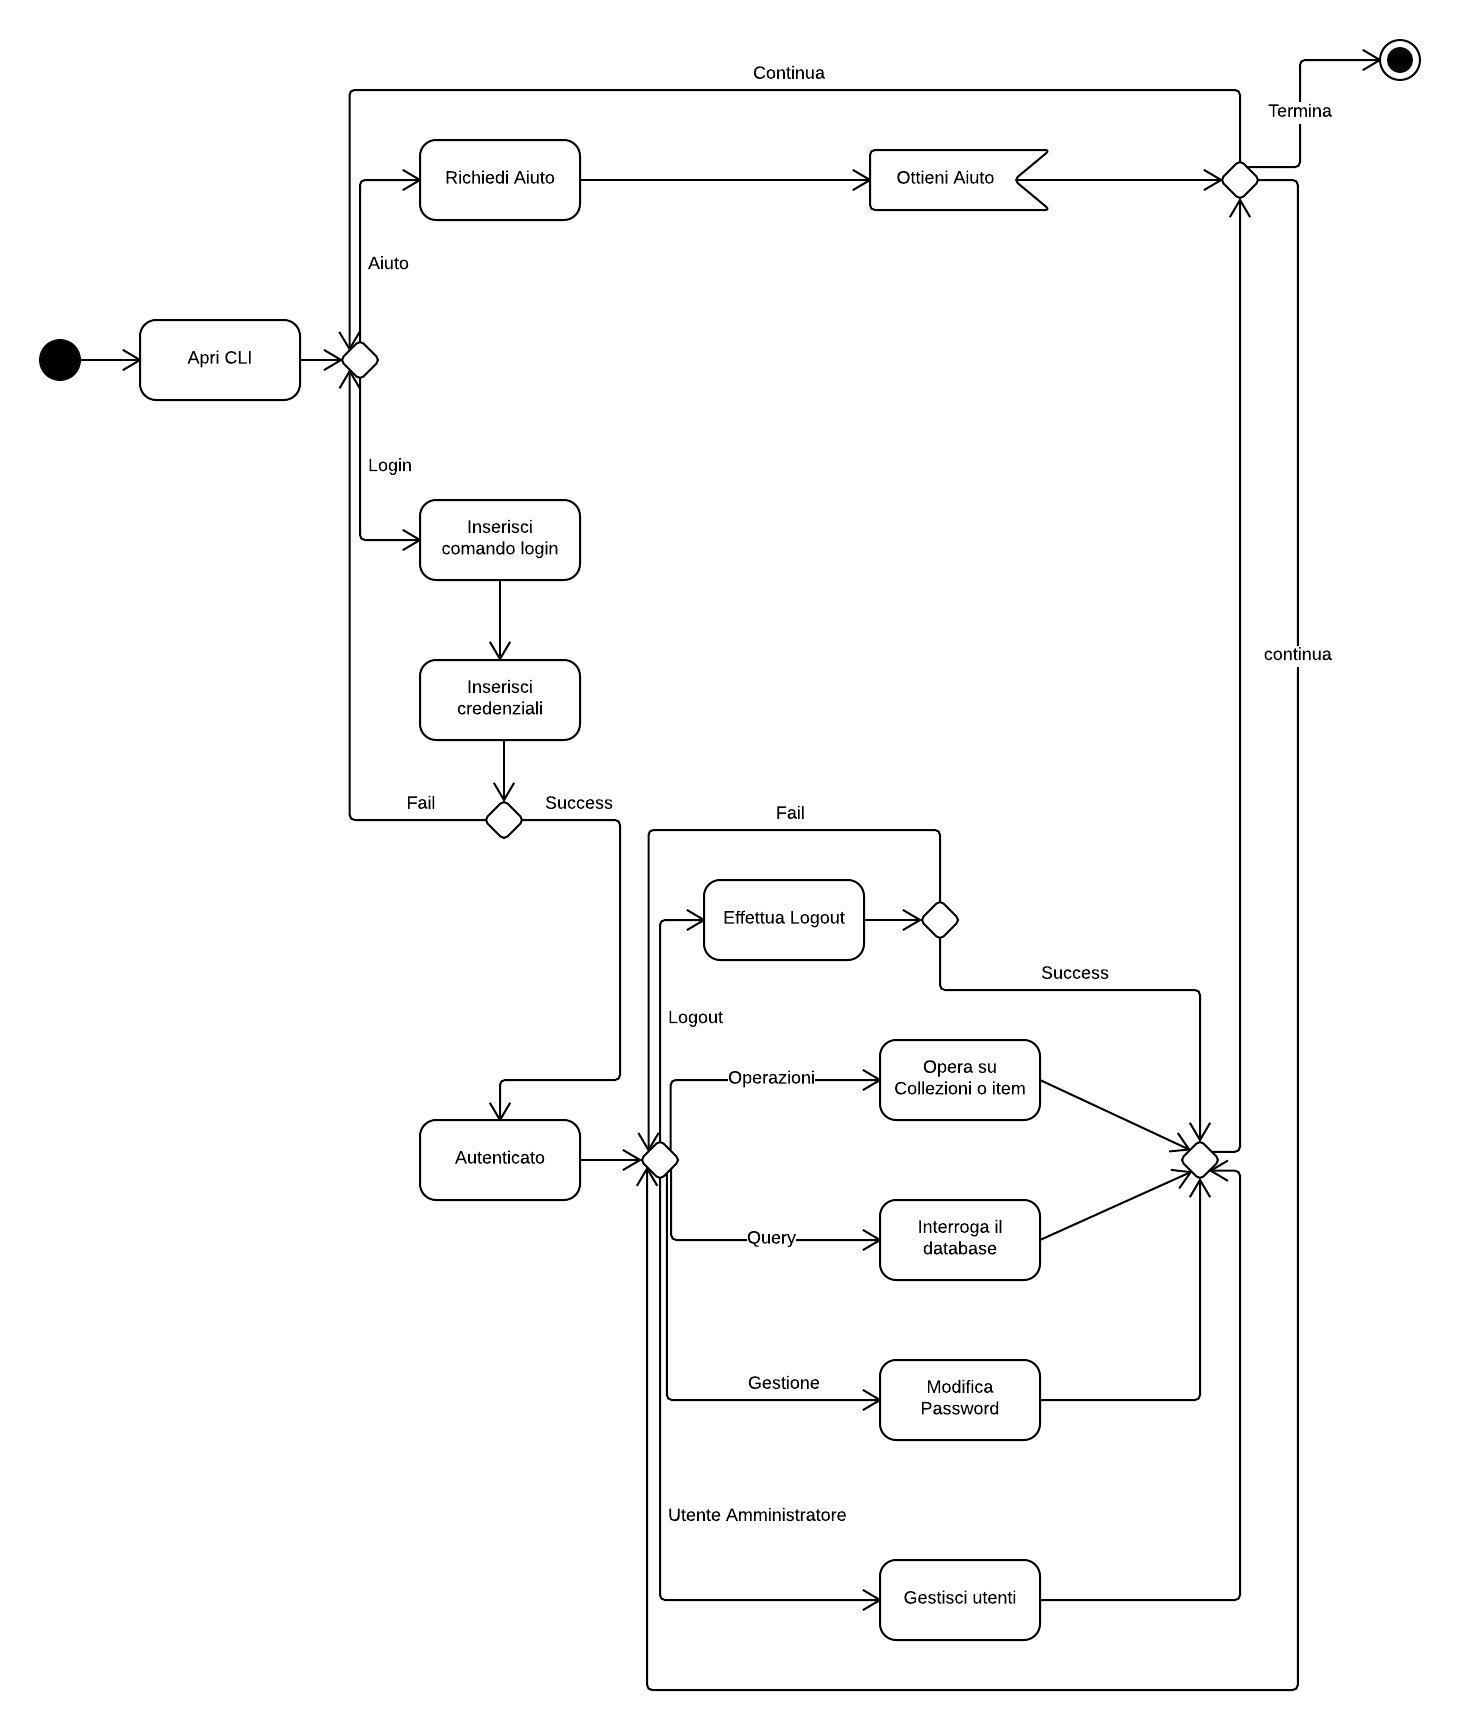
\includegraphics[width=0.8\textwidth, keepaspectratio]{img/diagrammiAttivita/visioneGenerale.jpeg}
		\caption{Diagrammi attività - Visione generale}
	\end{center}
\end{figure}

\subsection{Operazioni su collezioni e/o item}
\subsubsection{Creazione collezione}

Questo tipo di operazione permette di inserire una collezione all'interno del
database. Come si vede dal grafico che segue, l'utente dovrà inserire il
comando per la creazione della collezione, il nome della collezione stessa e i
suoi parametri. Una volta premuto il tasto invio, l'operazione andrà a buon
termine se l'utente ha scritto correttamente il comando altrimenti verrà
visualizzato un messaggio di errore.

\begin{figure}[H]
	\begin{center}
		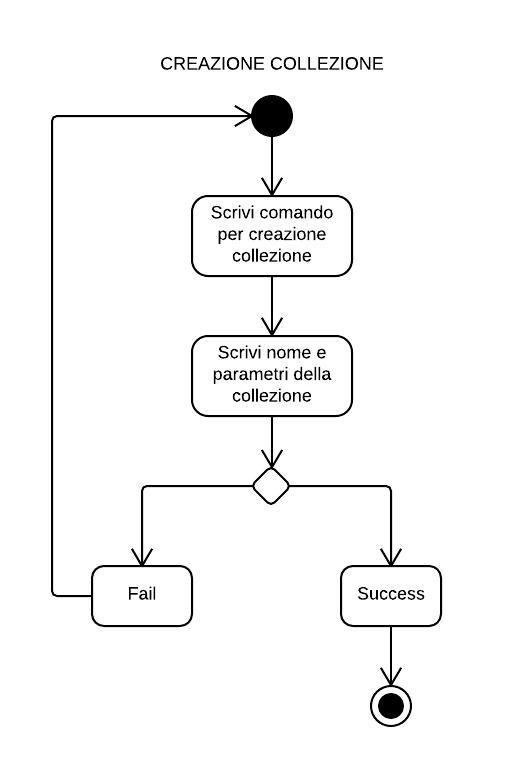
\includegraphics[width=0.3\textwidth, keepaspectratio]{img/diagrammiAttivita/creazioneCollezione.jpeg}
		\caption{Diagrammi attività - Creazione collezione}
	\end{center}
\end{figure}

\subsubsection{Cancellazione collezione}

Questo tipo di operazione permette di cancellare una collezione dal database.
Come si vede dal grafico che segue, l'utente dovrà inserire il comando per la
cancellazione di una collezione e il nome della collezione stessa. Una volta
premuto il tasto invio, l'operazione andrà a buon termine se l'utente ha
scritto correttamente il comando altrimenti verrà visualizzato un messaggio di
errore.

\begin{figure}[H]
	\begin{center}
		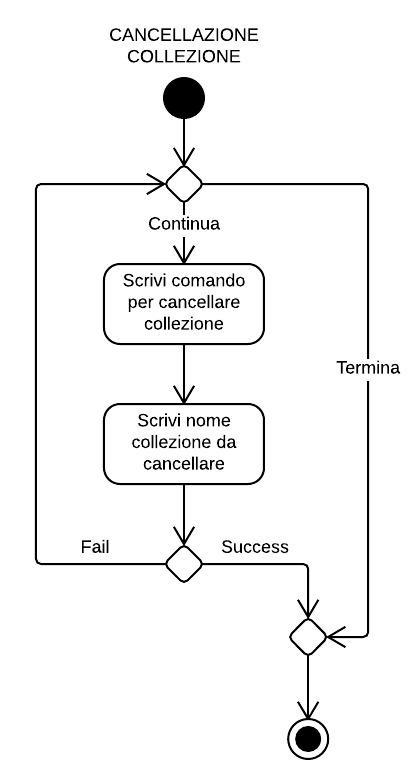
\includegraphics[width=0.3\textwidth, keepaspectratio]{img/diagrammiAttivita/cancCollezione.jpeg}
		\caption{Diagrammi attività - Cancellazione collezione}
	\end{center}
\end{figure}

\subsubsection{Visualizza collezioni}

Questo tipo di operazione permette di visualizzare le collezioni presenti
all'interno dal database. Come si vede dal grafico che segue, l'utente dovrà
inserire il comando per la visualizzazione delle collezioni. Una volta premuto
il tasto invio, l'operazione andrà a buon termine (ricevendo la lista delle
collezioni) se l'utente ha scritto correttamente il comando altrimenti verrà
visualizzato un messaggio di errore.

\begin{figure}[H]
	\begin{center}
		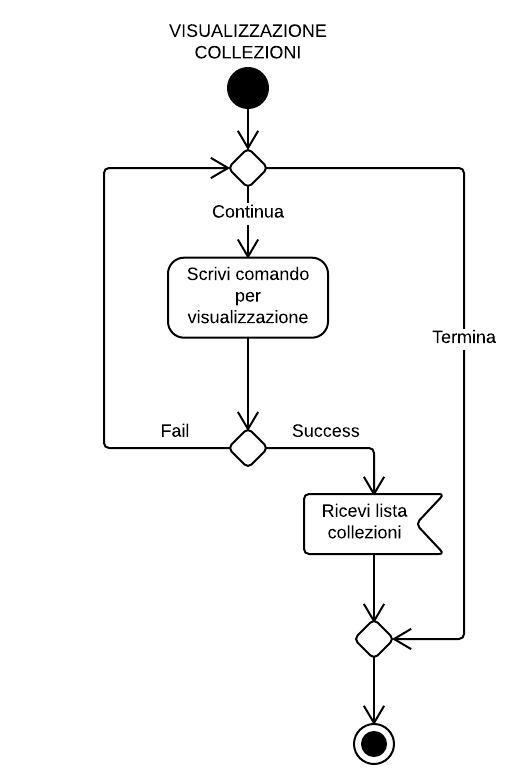
\includegraphics[width=0.3\textwidth, keepaspectratio]{img/diagrammiAttivita/visCollezione.jpeg}
		\caption{Diagrammi attività - Visualizzazione collezioni}
	\end{center}
\end{figure}

\subsubsection{Modifica nome collezione}

Questo tipo di operazione permette di modificare il nome di una collezione
presente nel database. Come si vede dal grafico che segue, l'utente dovrà
inserire il comando per la rinominazione della collezione, il nome della
collezione stessa e il nuovo nome per essa. Una volta premuto il tasto invio,
l'operazione andrà a buon termine se l'utente ha scritto correttamente il
comando altrimenti verrà visualizzato un messaggio di errore.

\begin{figure}[H]
	\begin{center}
		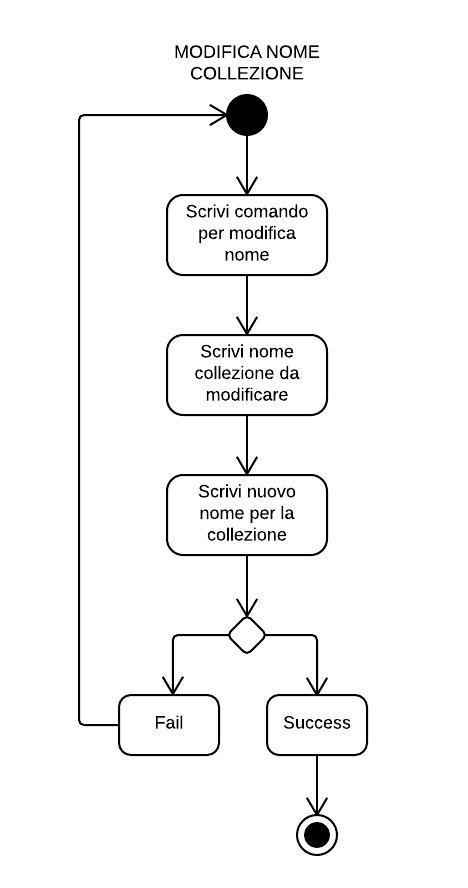
\includegraphics[width=0.3\textwidth, keepaspectratio]{img/diagrammiAttivita/modNomeCollezione.jpeg}
		\caption{Diagrammi attività - Modifica nome collezione}
	\end{center}
\end{figure}

\subsubsection{Inserimento item}

Questo tipo di operazione permette di inserire un item all'interno di una
collezione del database. Come si vede dal grafico che segue, l'utente dovrà
inserire il comando per l'inserimento item, il valore e parametri dell'item
stesso e il nome della collezione dove inserire l'item. Una volta premuto il
tasto invio, l'operazione andrà a buon termine (ricevendo la lista delle
collezioni) se l'utente ha scritto correttamente il comando altrimenti verrà
visualizzato un messaggio di errore.

\begin{figure}[H]
	\begin{center}
		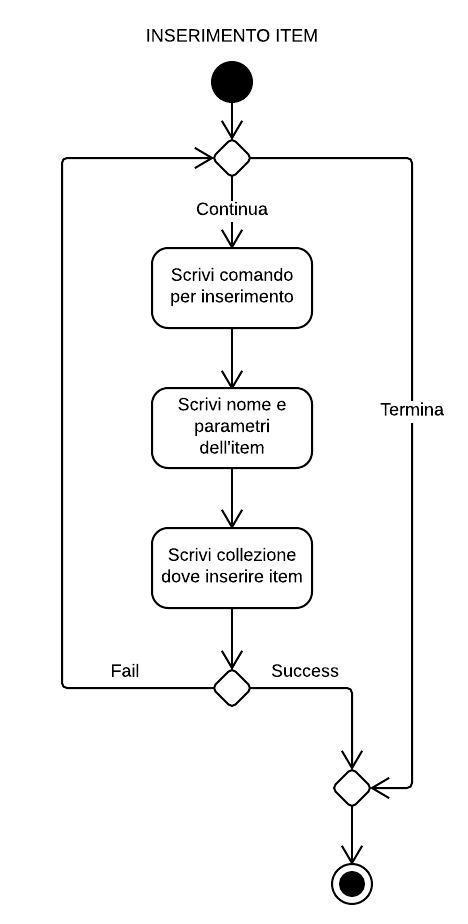
\includegraphics[width=0.3\textwidth, keepaspectratio]{img/diagrammiAttivita/inserimentoItem.jpeg}
		\caption{Diagrammi attività - Inserimento item}
	\end{center}
\end{figure}

\subsubsection{Rimozione item}

Questo tipo di operazione permette di rimuovere un item dall'interno di una
\gloss{collezione} del database. Come si vede dal grafico che segue, l'utente
dovrà inserire il comando per l'eliminazone di un item, il nome della
collezione da dove rimuovere l'item e il nome dell'item stesso. Una volta
premuto il tasto invio, l'operazione andrà a buon termine (ricevendo la lista
delle collezioni) se l'utente ha scritto correttamente il comando altrimenti
verrà visualizzato un messaggio di errore.

\begin{figure}[H]
	\begin{center}
		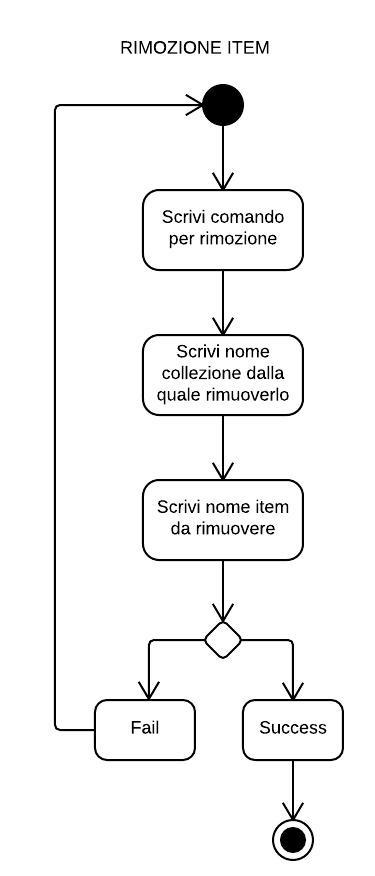
\includegraphics[width=0.3\textwidth, keepaspectratio]{img/diagrammiAttivita/rimozioneItem.jpeg}
		\caption{Diagrammi attività - Rimozione item}
	\end{center}
\end{figure}

\subsubsection{Aggiunta collaboratore}

Questo tipo di operazione permette di aggiungere un \gloss{collaboratore} ad
una collezione presente nel database. Come si vede dal grafico che segue,
l'utente dovrà inserire il comando per l'aggiunta di un collaboratore ad una
collezione, lo username del collaboratore e il nome della collezione alla
quale aggiungerlo. Una volta premuto il tasto invio, l'operazione andrà a buon
termine se l'utente ha scritto correttamente il comando altrimenti verrà
visualizzato un messaggio di errore.

\begin{figure}[H]
	\begin{center}
		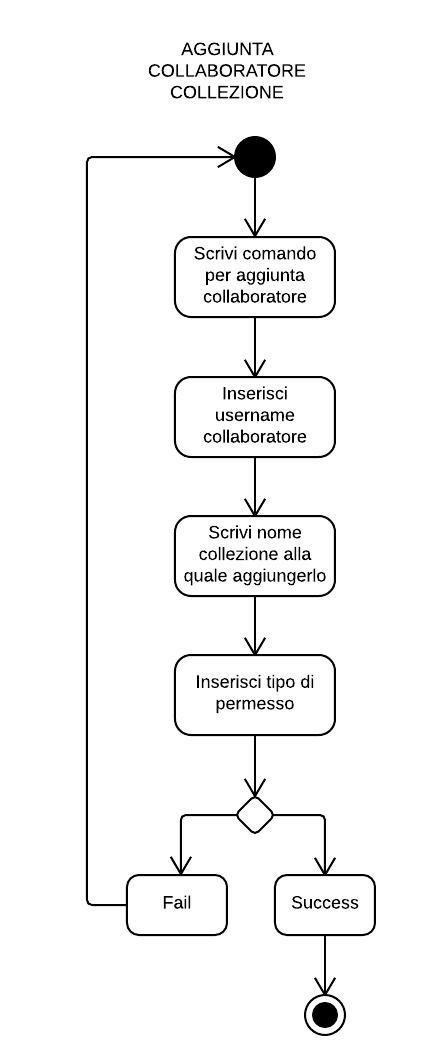
\includegraphics[width=0.3\textwidth, keepaspectratio]{img/diagrammiAttivita/aggCollaboratore.jpeg}
		\caption{Diagrammi attività - Aggiunta collaboratore}
	\end{center}
\end{figure}

\subsubsection{Rimozione collaboratore}

Questo tipo di operazione permette di rimuovere un collaboratore da una
collezione presente nel database. Come si vede dal grafico che segue, l'utente
dovrà inserire il comando per la rimozione di un collaboratore da una
collezione, lo username del collaboratore e il nome della collezione dalla
quale rimuoverlo. Una volta premuto il tasto invio, l'operazione andrà a buon
termine se l'utente ha scritto correttamente il comando altrimenti verrà
visualizzato un messaggio di errore.

\begin{figure}[H]
	\begin{center}
		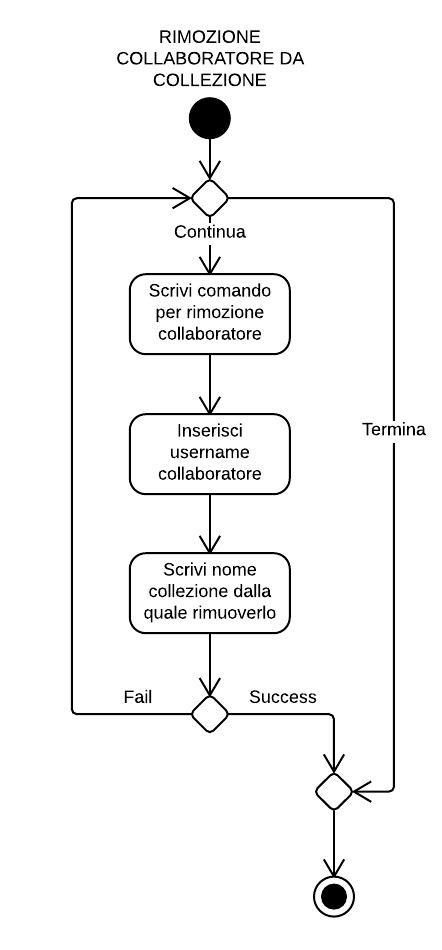
\includegraphics[width=0.3\textwidth, keepaspectratio]{img/diagrammiAttivita/rimozioneCollaboratore.jpeg}
		\caption{Diagrammi attività - Rimozione collaboratore}
	\end{center}
\end{figure}

\subsubsection{Import}

Questo tipo di operazione permette di importare nel database collezioni o item
tramite file \gloss{JSON}. Come si vede dal grafico che segue, l'utente dovrà
inserire il comando per l'importazione e il path che porta al file desiderato.
Una volta premuto il tasto invio, l'operazione andrà a buon termine se
l'utente ha scritto correttamente il comando altrimenti verrà visualizzato un
messaggio di errore.

\begin{figure}[H]
	\begin{center}
		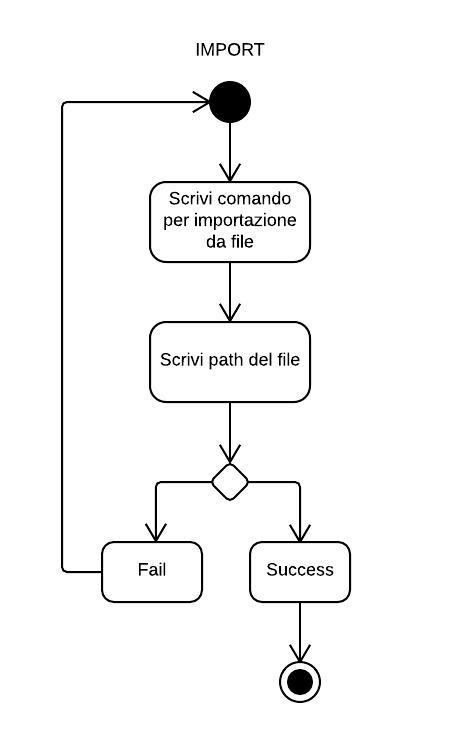
\includegraphics[width=0.3\textwidth, keepaspectratio]{img/diagrammiAttivita/import.jpeg}
		\caption{Diagrammi attività - Import}
	\end{center}
\end{figure}

\subsection{Interrogazione del database}

Questo tipo di operazione permette di interrogare il database tramite delle
query. Come si vede dal grafico che segue, l'utente dovrà inserire il comando
per l'interrogazione del database e i parametri per la ricerca. Una volta
premuto il tasto invio, l'operazione andrà a buon termine se l'utente ha
scritto correttamente il comando, ricevendo il risultato della query,
altrimenti verrà visualizzato un messaggio di errore.

\begin{figure}[H]
	\begin{center}
		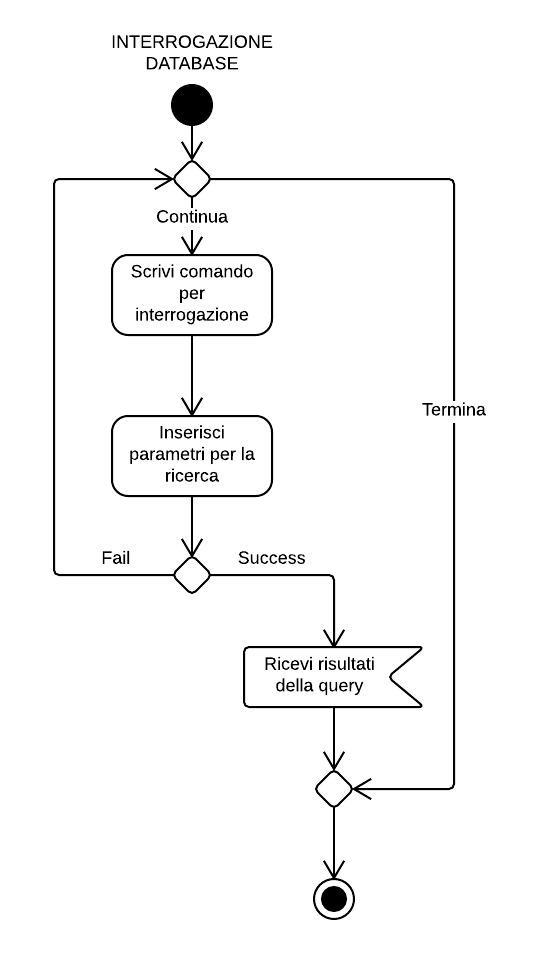
\includegraphics[width=0.3\textwidth, keepaspectratio]{img/diagrammiAttivita/query.jpeg}
		\caption{Diagrammi attività - Interrogazione del database}
	\end{center}
\end{figure}

\subsection{Modifica password}

Questo tipo di operazione permette di modificare la propria password. Come si
vede dal grafico che segue, l'utente dovrà inserire il comando per la modifica
della password, la vecchia password, la nuova password e confermare
quest'ultima. Una volta premuto il tasto invio, l'operazione andrà a buon
termine se l'utente ha scritto correttamente il comando altrimenti verrà
visualizzato un messaggio di errore.

\begin{figure}[H]
	\begin{center}
		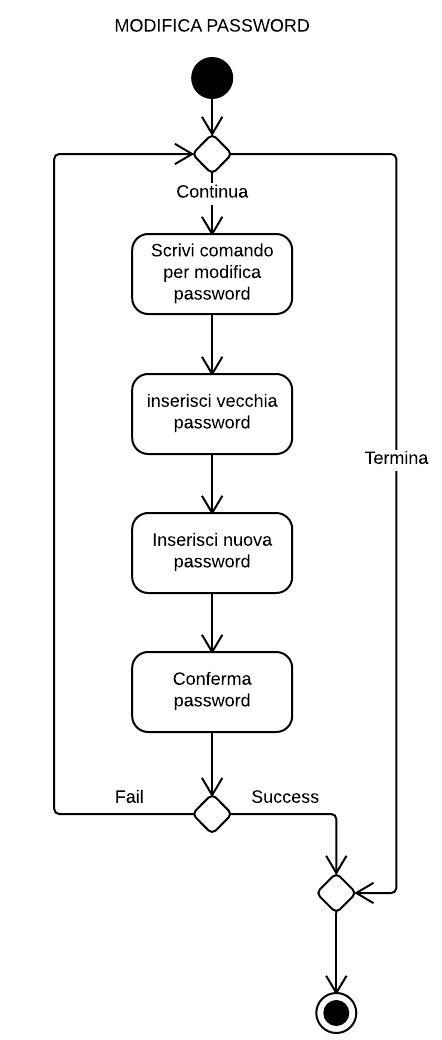
\includegraphics[width=0.3\textwidth, keepaspectratio]{img/diagrammiAttivita/modificaPsw.jpeg}
		\caption{Diagrammi attività - Modifica password}
	\end{center}
\end{figure}

\subsection{Gestione utenti}

La gestione utenti, possibile solo ad un utente amministratore, prevede la
possibilità di aggiungere o rimuovere un utente dal database e la possibilità
di resettare la password di un utente. Per aggiungere o rimuovere un utente,
l'amministratore dovrà inserire il rispettivo comando, lo username dell'utente
da aggiungere/rimuovere dal database e una conferma. Per resettare la password
di un utente, l'amministratore dovrà scrivere il comando per il reset della
password, lo username dell'utente interessato e una conferma. Una volta
premuto il tasto invio, le operazione andranno a buon termine se l'utente ha
scritto correttamente il comando altrimenti verrà visualizzato un messaggio di
errore.

\begin{figure}[H]
	\begin{center}
		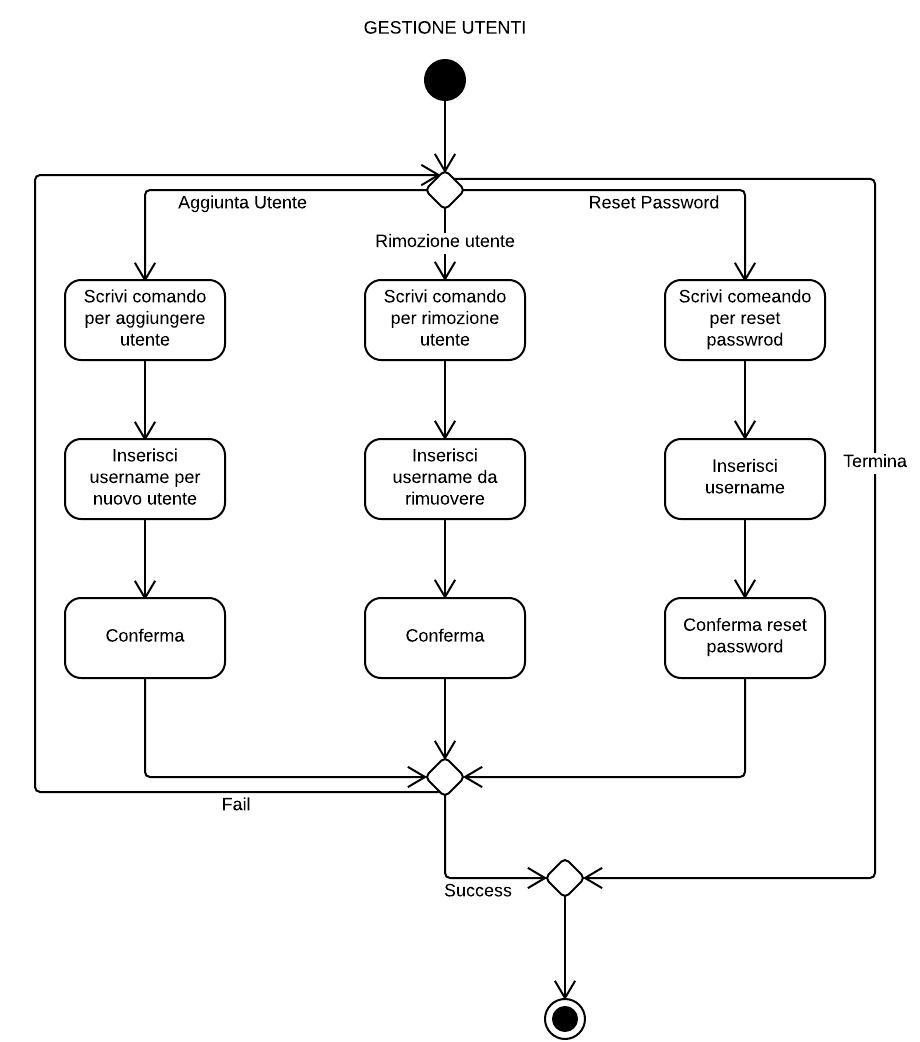
\includegraphics[width=0.3\textwidth, keepaspectratio]{img/diagrammiAttivita/gestioneUtenti.jpeg}
		\caption{Diagrammi attività - Gestione utenti}
	\end{center}
\end{figure}

\section{Design Pattern}

\subsection{Stime di fattibilità e di bisogno di risorse}

\section{Tracciamento}

\subsection{Tracciamento componenti - requisiti}

\subsection{Tracciamento requisiti - componenti}

\appendix
\section{Descrizione design pattern}
\listoftables
\listoffigures
\end{document}